% \documentclass{ksp}
\documentclass{../../../ksp}

\usepackage{graphicx}
\graphicspath{ {./} }

\title{KSP 35--3--2}
\author{Daniel Culliver}
\date{Únor 2023}

\begin{document}

\maketitle

\section*{Řešení}

Tak samozřejmě první řešení které nás napadá je hrubě projít každou mističku pro každého člověka.
Toto jednoduché řešení vyjde na složitost $\BigO(N \cdot K)$, což není až tak hrozné.
Ale existuje určitě lepší řešení.

Jaké je tedy to lepší řešení?
No, je to pomocí něčemu čemu se říká intervalové stromy, o kterých jsem se dozvěděl z knížky \emph{Průvodce labyrintem algoritmů}.

Prvím krokem této řešení je, že si nejprve uspořádáme všechny mističky podle toho, jakou koncentraci čaje vytvoří.
Toto bude vyžadovat $\BigO(K\log{K})$ kroků.

Poté vytvoříme tedy ten intervalový strom. Je potřeba uvažovat o mističkách jako objekty, které drží více informací.
Přesněji jejich původní pořadí při načtení ze vstupu (což bychom pravděpodobně potřebovali při praktickém řešením úlohy),
poté ještě počet listí na vystelení mističky ($L_i$) a koncentraci čaje, kterou mističkou vytvoříme ($C_i$).

Mističky máme seřazené podle jejich koncentraci, ale intervalový strom bude ukládat počet minimální počet listí na nějaké intervaly.
Strom bude binární, proto bude velmi jednoduché ho uložit do pole.
Tvorba stromu vyžaduje $\BigO(K)$ kroků (přesněji $2K$), protože můžeme začít ze zdola (z původního pole) a postupně ukládat prvky výš ve stromě,
tedy blíž k začátku pole do kterého strom ukládáme.

Přes strom budeme tedy schopni dotázat na nejmenší počet listí na vystelení misky pro daný interval v $\BigO(\log{K})$ čase.

Příkladem stromu je tohle (omluvte prosím velmi nízkou kvalitu obrázku):

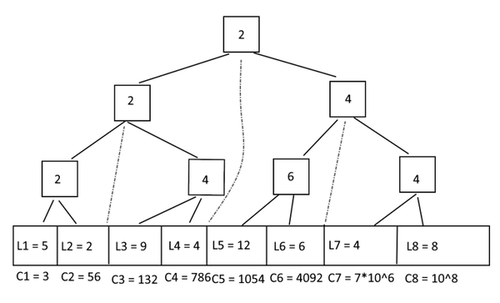
\includegraphics{strom2}

Protože budeme dotazovat na strom přes koncentraci a ne indexy, každý vrchol nad původním polem
Jednak, každý vrchol bude muset mít uložené hodnoty koncentrace nejvíce vpravo a nejvíce vlevo,
aby se mohlo zjistit \emph{identita} intervalů.

Podle přikladu v obrázky by tohle znamenalo, že kdybychom se ptali na interval $\langle 2; 10^9 \rangle$,
tak rovnou vrátíme nejvyšší vrchol, protože bude podmnožinou našeho dotazu, ale zároveň bude obsahovat všechny
možné mističky pro ten dotaz.

Další hodnoty, které vrcholy budou muset mít uložené (protože jejich uložení zabere konstatní čas při tvoření stromu)
budou hodnoty nejblíže ke středu (t.j.\ ty pod příslušným vrcholem).
Toto umožní, abychom mohli správě rozdělovat dotazy na více vrcholů v stromu.

Například dotaz $\langle 4; 10^9 \rangle$ zavolá dvě dotazy, první na levého podstromu $\langle 4; 786 \rangle$
a druhý na pravý podstrom $\langle 1054; 10^9 \rangle$

Teď už jsme připravení abychom mohli dotazovat na náš strom v $\BigO(\log{K})$ času.
Ještě si uvedeme pseudokód dotazu:

\begin{algorithm*}
    \caption{DotazIntervalů}
    \begin{algorithmic}
        \Require{index vrcholu $v$ ve stromu, interval vrcholu $\langle a; b \rangle$, hledaný interval $\langle i; j \rangle$ }
        \If{$i \leq a$ and $j \geq b$}
            \State{return $v$}
        \EndIf{}
        \State{$S_l \gets$ hodnota hned vlevo od `středu' vrcholu \Comment{v příkladu by pro v=0 rovnalo 786}}
        \State{$S_r \gets$ hodnota hned vpravo od `středu' vrcholu \Comment{v příkladu by pro v=0 rovnalo 1054}}
        \If{$j \leq S_r$}
            \State{return DotazIntervalů (2$v$, $\langle a; S_l \rangle$, $\langle i; j \rangle$)}
        \ElsIf{$i \geq S_l$}
            \State{return DotazIntervalů ($2v+1$, $\langle S_r; b \rangle$, $\langle i; j \rangle$)}
        \Else{}
            \State{return DotazIntervalů (2$v$, $\langle a; S_l \rangle$, $\langle i; S_l \rangle$)}
            \State{return DotazIntervalů ($2v+1$, $\langle S_r; b \rangle$, $\langle i; S_r \rangle$)}
        \EndIf{}
        \Ensure{All intervals that $\langle i; j \rangle$ contains}
    \end{algorithmic}
\end{algorithm*}

Jaká je teda složitost tohoto řešení?
No, nejprve si vypočítáme časovou složitost.
Třídení mističek je $\BigO(K\log{K})$, tvoření stromu je $\BigO(K)$ a všechny dotazy budou
$\BigO(N\log{K})$. Celkově to tedy vyjde na $\BigO(K\log{K} + N\log{K})$.

Je důležité si ale poznamenat, že toto řešení vlastně ani nemusí být vždycky lepší než jednoduché, hrubé řešení uvedené na začátku.
Rovnou změníme obecné $\log{K}$ na $\log_2{K}$, které je přesnější pro tyto výpočty.
\begin{equation}
    \begin{split}
        N \cdot K & < K\log_2{K} + N\log_2{K}\\
        1 & < \frac{\log_2{K}}{N} + \frac{\log_2{K}}{K}
    \end{split}
\end{equation}
Už jenom na této nerovnici můžeme zpozorovat, že pro $N \leq \log{K}$ bude intevalový storm horší.
Samozřejmě, když se budou obě hodnoty blížit nekonečnu, tak intervalový strom je mnohem lepší, jen je ale
důležité si pamatovat, že pro velmi velké $K$ může existovat ne úplně malé $N$, pro který bychom preferovali
jednoduchý, hrubý algoritmus.

A teď si ještě rychle na konci spočítáme prostorovou složitost. Nejvíce paměti bude zabírat náš strom,
takže započítáme jenom jeho: $\BigO(K)$ (přesněji to vyjde okolo $6K$)

\end{document}